%! Author = alana
%! Date = 09/09/2022

% Preamble
\documentclass[a4paper, 11pt]{article}

% Packages
\usepackage[brazil]{babel}
\usepackage[utf8]{inputenc}
\usepackage{amsmath, lmodern, amsthm, amstext, ebezier, amscd}
\usepackage{graphicx}
\usepackage[a4paper, left=2.5cm, right=2.5cm, top=2.5cm, bottom=2.5cm]{geometry}
\usepackage{setspace}
\usepackage{lipsum} \doublespacing
\usepackage{listings}
\usepackage{color}
\usepackage{indentfirst}
\usepackage{hyperref}
\usepackage{lstmisc}
\usepackage{pythontex}
\usepackage{chemfig}
\usepackage{xymtex}



% Document
\begin{document}
    \thispagestyle{empty} % Remove page number from first page to title page

    \begin{center}
        \parbox{3cm}{
\includegraphics[scale=1]{logo_ufpa}} \\
        {\vspace {1.0cm}}
        {\Large \uppercase {Universidade Federal do Pará}}\\
        {\Large \uppercase {Instituto de Ciências Exatas e Naturais - ICEN}}\\
        \vspace{3cm}
        {\Large \uppercase {Faculdade de Química - FAQUI}}\\
        {\Large \uppercase {Laboratório de Química Analítica Quantitativa 2022.2} }\\
        \vspace{3cm}
        {\Large \bf \uppercase {Relatório de Prática 5: Lei dos Gases - Reação do Carbonato de Cálcio com Ácido Clorídrico}}\\
        {\Large \bf \uppercase {Prof. Dr. Carlos Antonio Neves}}\\
        \vspace{3cm}
        {\Large \uppercase {Alan Henrique Pereira Miranda - 202102140072}}\\
        {\Large \uppercase {Gabriel Cruz de Oliveira - 202102140055}}\\
        {\Large \uppercase {Paloma Gama da Silva - 202102140029}}\\
        {\Large \uppercase {Silvio Farias Leal - 202102140035}}\\
        \vspace{0.5cm}
        {\Large  {Belém-PA \\ 2022}}
    \end{center}

    \newpage
    \section{Introdução}\label{sec:introducao}

    \indent Este experimento visa demonstrar a validade da relação de Clayperon, ou também conhecida como lei dos gases ideais. O experimento utiliza-se da reação do Carbonato de Cálcio com o Ácido Clorídrico\@.\\
    \indent Este experimento se baseia na reação entre um sal inorgânico e um ácido forte. O Carbonato de cálcio é muito utilizado na industria farmacêutica como um antiácido de ação rápida, permitindo uma rápida demonstração de uma reação química \@.\\

    \section{Objetivos}\label{sec:objetivos}

    \indent - Verificar experimentalmente a Lei dos Gases; \\
    \indent - Determinar o volume de gás produzido na reação do Carbonato de Cálcio com Ácido Clorídrico\@.

    \section{Materiais e Métodos}\label{sec:materiais_metodos}
    \subsection{Materiais}\label{sec:materiais}
    \indent Os materiais e reagentes utilizados neste experimento são os seguintes\@:
    \subsubsection{Materiais Utilizados}\label{sec:materiais_utilizados}
    \begin{itemize}
        \item Garra Metálica\@.
        \item Mangueira de Borracha\@.
        \item Proveta de $50ml$\@.
        \item Rolha de Madeira\@.
        \item Suporte Universal\@.
        \item Tubo de Ensaio Graduado\@.
        \item Pipeta\@.
        \item Kitassato de $250ml$\@.
        \item Bequer $500ml$\@.
        \item Balança Analítica\@.
    \end{itemize}
    \doublespacing
    \subsubsection{Reagentes Utilizados}\label{sec:reagentes_utilizados}
    \begin{itemize}
        \item Carbonato de Cálcio\@.
        \item Água\@.
        \item Ácido Clorídrico\@.
    \end{itemize}
    \doublespacing

    \subsection{Procedimentos}\label{sec:procedimentos}
    \subsubsection{Preparação da solução de sulfato de cobre II}\label{sec:preparacao_solucao}
    \begin{enumerate}
        \item Preparação da Balança e do Bequer utilizado para quantificar a massa de carbonato de cálcio\@.
        \item Obtenção da massa necessária, $0.190g$, de carbonato de cálcio\@.
        \item Preparação do bequer de $500ml$, da mangueira de borracha e do tubo de ensaio graduado com água em uma quantidade suficiente\@.
        \item Transferência da massa de carbonato de cálcio para o kitassato\@.
        \item Separação de $20ml$ de ácido clorídrico com uma pipeta\@.
        \item Adição do ácido clorídrico ao kitassato de modo a não entrar em contato com o carbonato de cálcio\@.
        \item Vedação do kitassato com a rolha de madeira para que a emissão de gases da reação seja armazenada\@.
        \item Mistruar o ácido clorídrico com o carbonato de cálcio\@.
    \end{enumerate}
    \doublespacing

    \subsubsection{Determinação da quantidade de gás produzido na reação}\label{sec:determinacao_concentracao}
    \indent O procedimento de determinação da concentração da solução obtida passa pela utilização da seguinte equação:\\
    \begin{equation}
        \label{eq:equacao_concentracao}
        P.V = n.R.T
    \end{equation}

    \indent Onde $P$ é a Pressão Atomosférica, $n$ é o número de mols de dióxido de carbono produzido, $R$ é a constante dos gases ideais, $T$ é a temperatura e $V$ é o volume do gás\@.\\

    \indent Dados iniciais:
    \begin{itemize}
        \item Massa de carbonato de cálcio: $0.190g$\@.
        \item Massa molar do carbonato de cálcio: $123.55 g/mol$ \@.
        \item Volume de água: $0.5L$ \@.
        \item Massa molar do ácido clorídrico: $36.458g/mol$\@.
        \item Constante dos gases ideais: $0.082 L.ATM/K.mol$
    \end{itemize}

    \indent Desta forma, temos:
    \begin{center}
        \begin{equation}
            \label{eq:equacao_concentracao}
            P.V = n.R.T

            (1 ATM) . V = n . (0,082 L.ATM/K.mol) . (295,65K)

            C = \frac{m1}{V}
            = \frac{2.5212g}{0.10L}
            = 0.100967\frac{g}{L}

        \end{equation}
    \end{center}

    \subsection{Procedimentos aplicados em laboratório}\label{sec:procedimentos_laboratorio}
    \indent O procedimento inicial é a preparação da balança e do bequer para quantificar a massa da solução\@. Tal processo
    se deu com o procedimento de ``targ'' da balança com o peso do becker, como podemos verificar na imagem a seguir\@: \\
    \begin{center}
        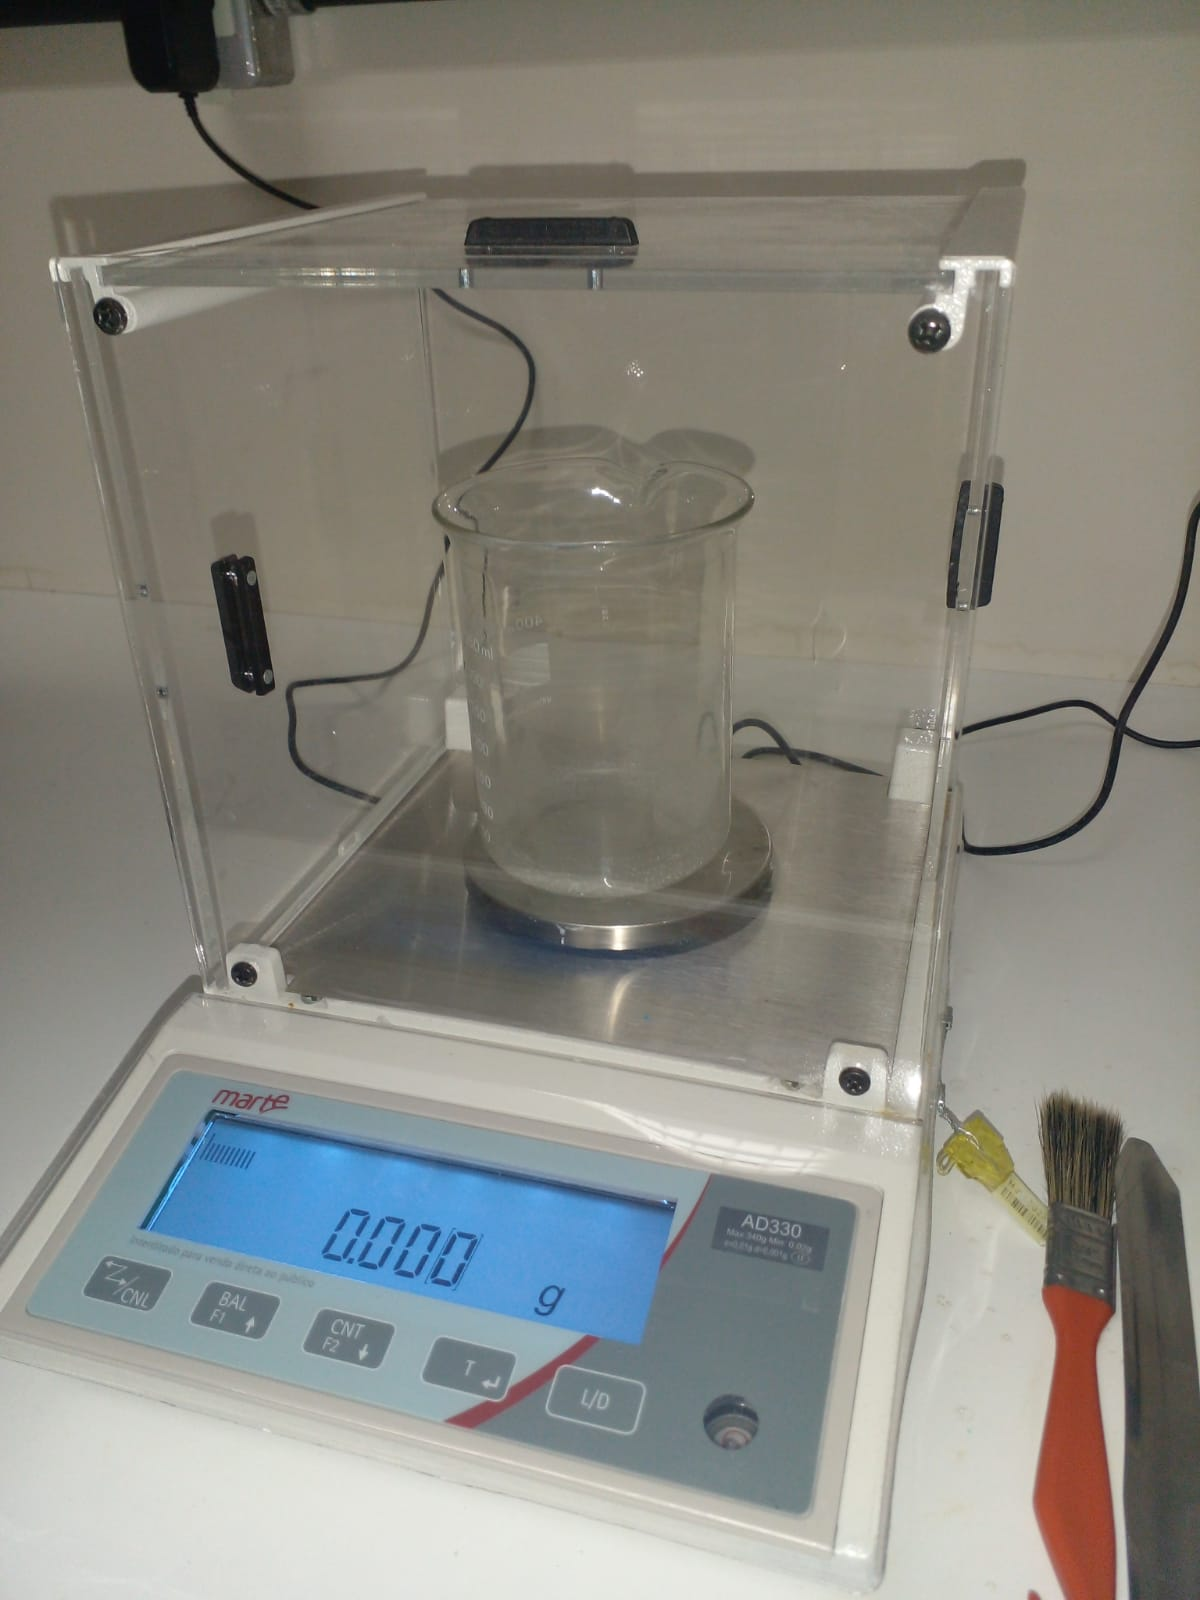
\includegraphics[scale=0.2]{03. preparo da balanca.jpeg}\\
        \singlespacing
        \textbf{Figura 1}: Preparo da balança\@.
    \end{center}
    \doublespacing

    \indent O preparo da solução iniciou com a quantificação da massa, que no caso foi de $2.521g$, de sulfato de cobre II\@.\\
    \begin{center}
        \parbox{7cm}{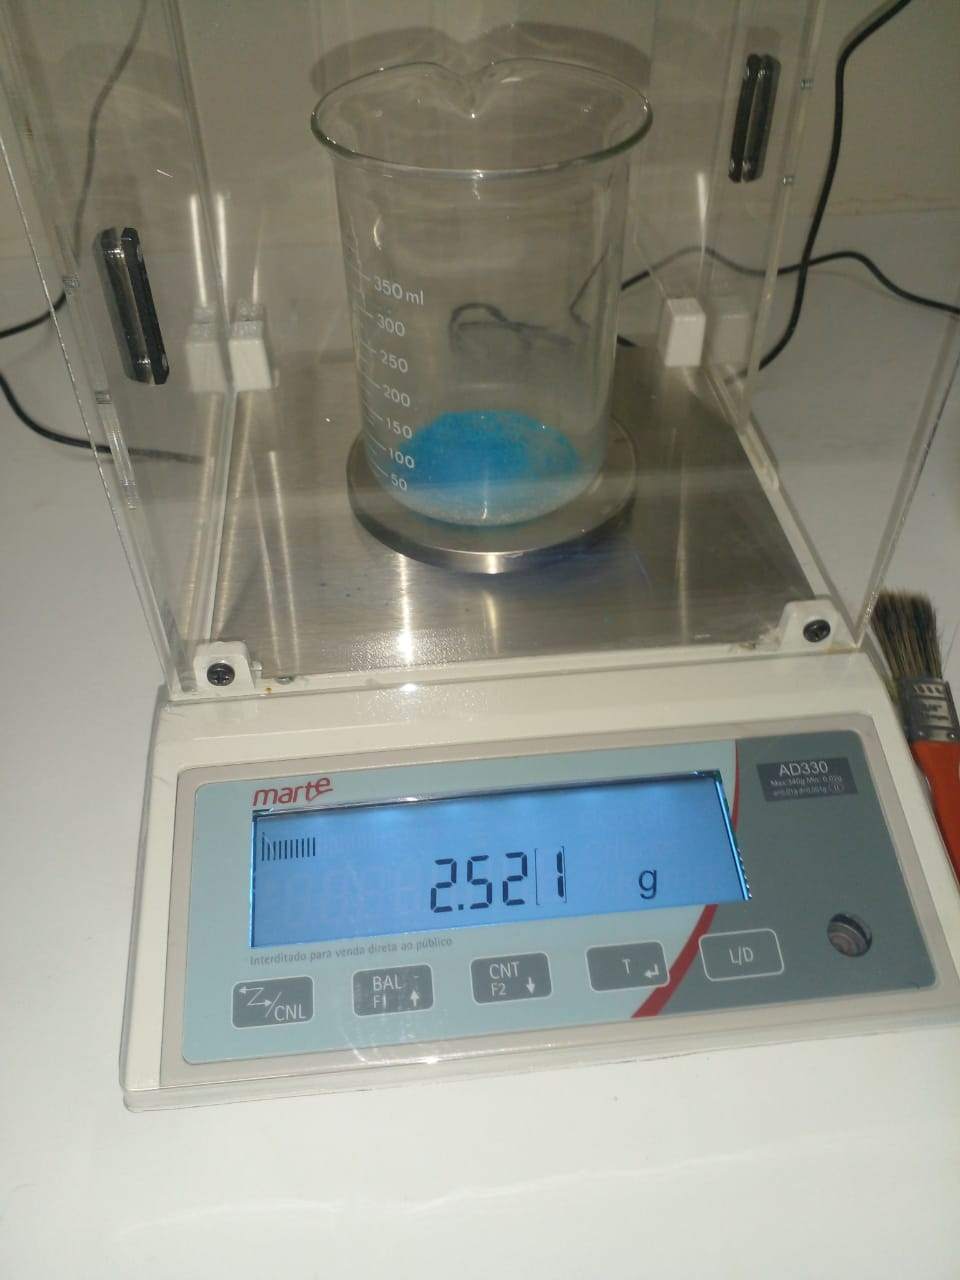
\includegraphics[scale=0.2]{02. massa_utilizada.jpeg}}\\
        \singlespacing
        \textbf{Figura 2}: Massa de sulfato de cobre II\@.
    \end{center}
    \doublespacing

    \indent Após a quantificação da massa, foi necessário preparar o balão volumétrico, o Funil e a Pisseta com água destilada\@.
    É necessário verificar a presença de umidade na vidraçaria utilizada, uma vez que tal condição pode afetar o procedimento\@.\\
    Podemos verificar na imagem a seguir que o Funil e o balão estavam secos, e a Pisseta contendo $200ml$ de água destilada\@:

    \begin{center}
        \parbox{7cm}{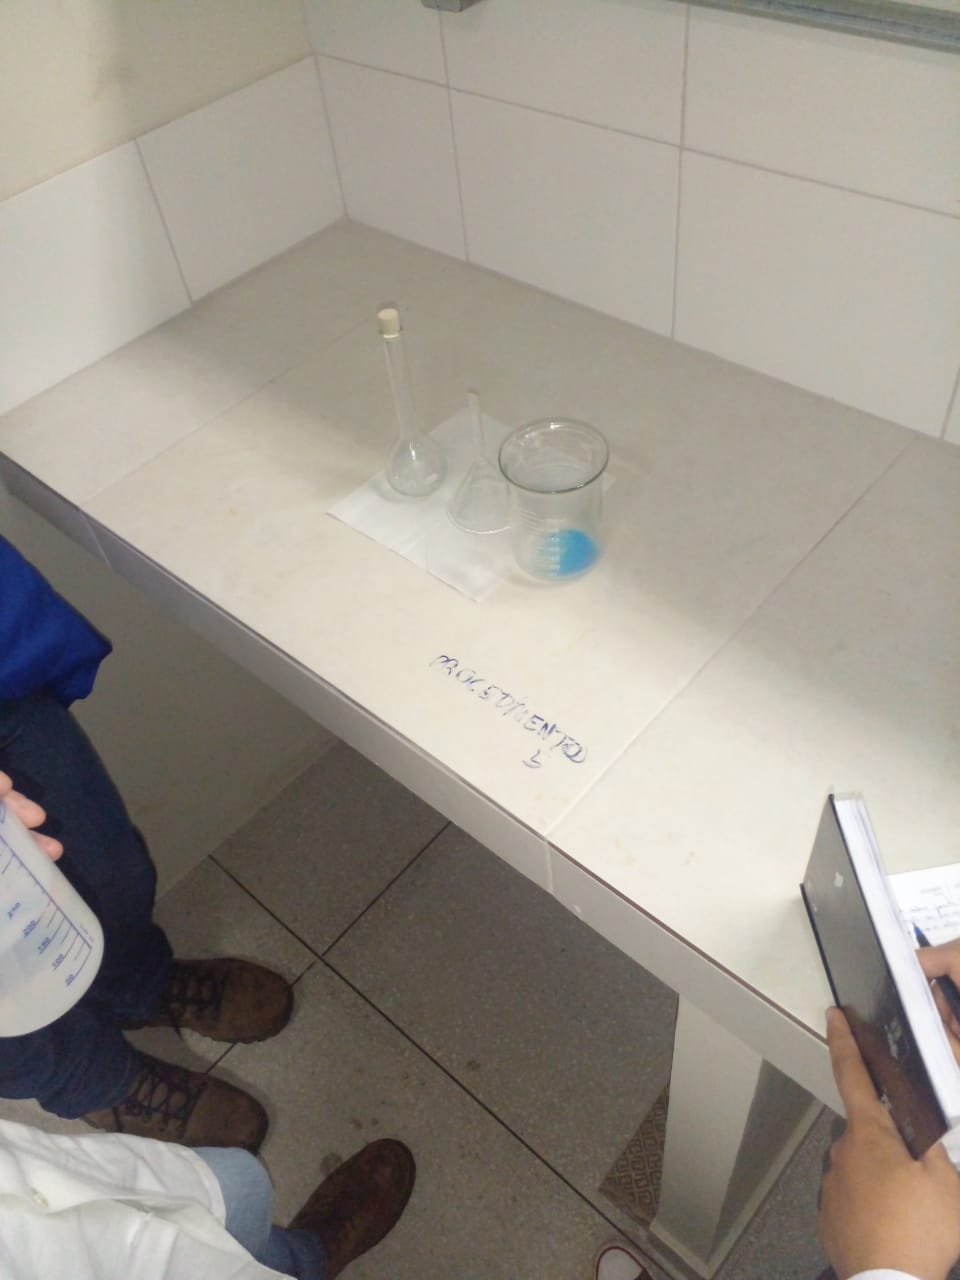
\includegraphics[scale=0.2]{01. instrumentos utilizados.jpeg}}\\
        \singlespacing
        \textbf{Figura 3}: Inicio do preparo da solução\@.
    \end{center}
    \doublespacing

    \indent Logo após a preparação dos instrumentos, foi adicionado água destilada no becker para a solubilização do sulfato de cobre II,
    onde este foi agitado até que fosse totalmente solubilizado\@.
    verificou-se também, o encaixe do funil com o bocal do balão volumétrico, para que este não fosse totalmente vedado durante a
    adição do concentrado de sulfato de cobre II\@.\\

    \begin{center}
        \begin{tabular}{c c}
            \parbox{7cm}{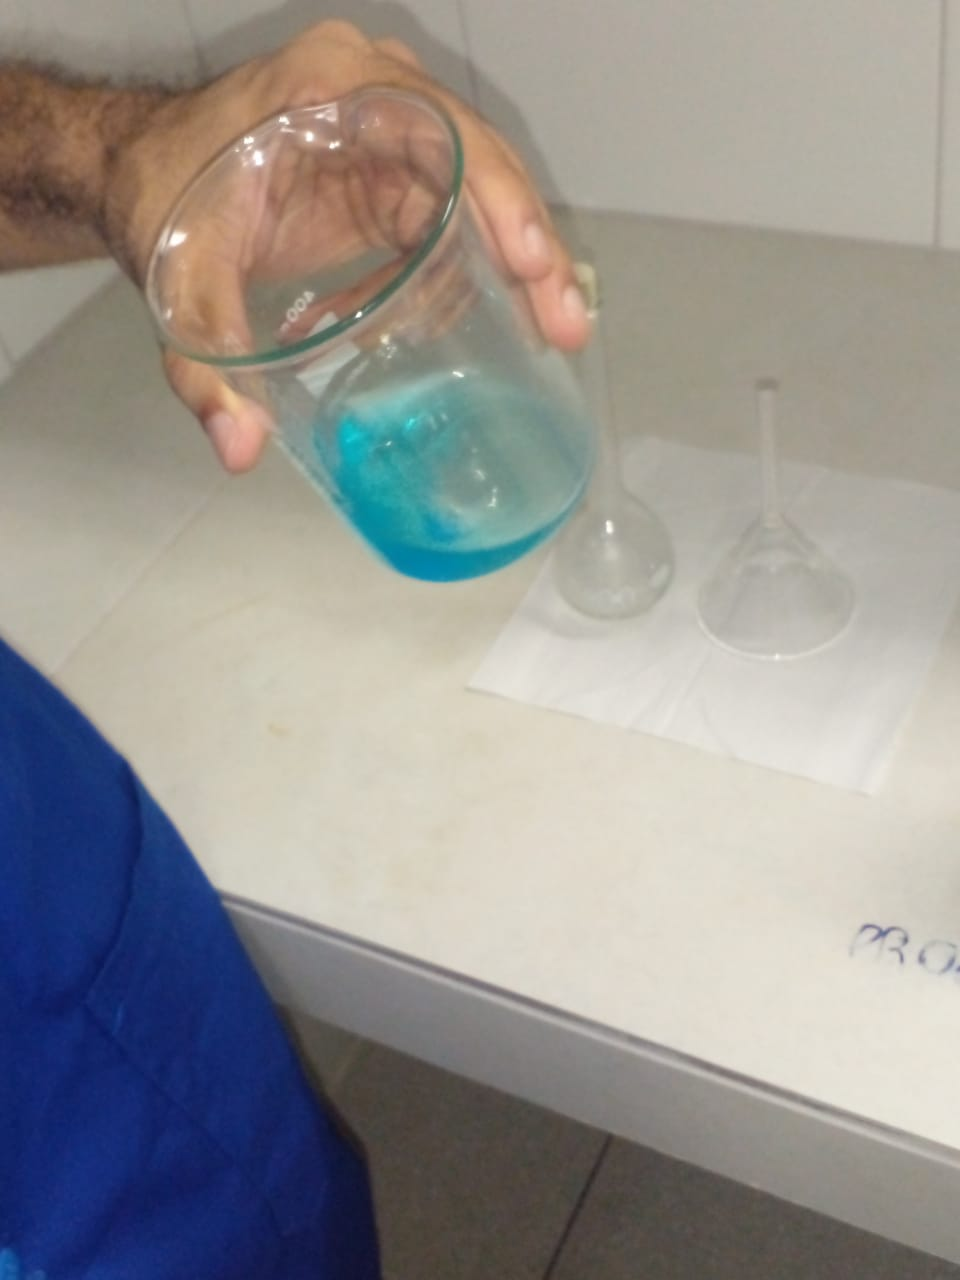
\includegraphics[scale=0.2]{05. solubilizacao.jpeg}}
            & \parbox{7cm}{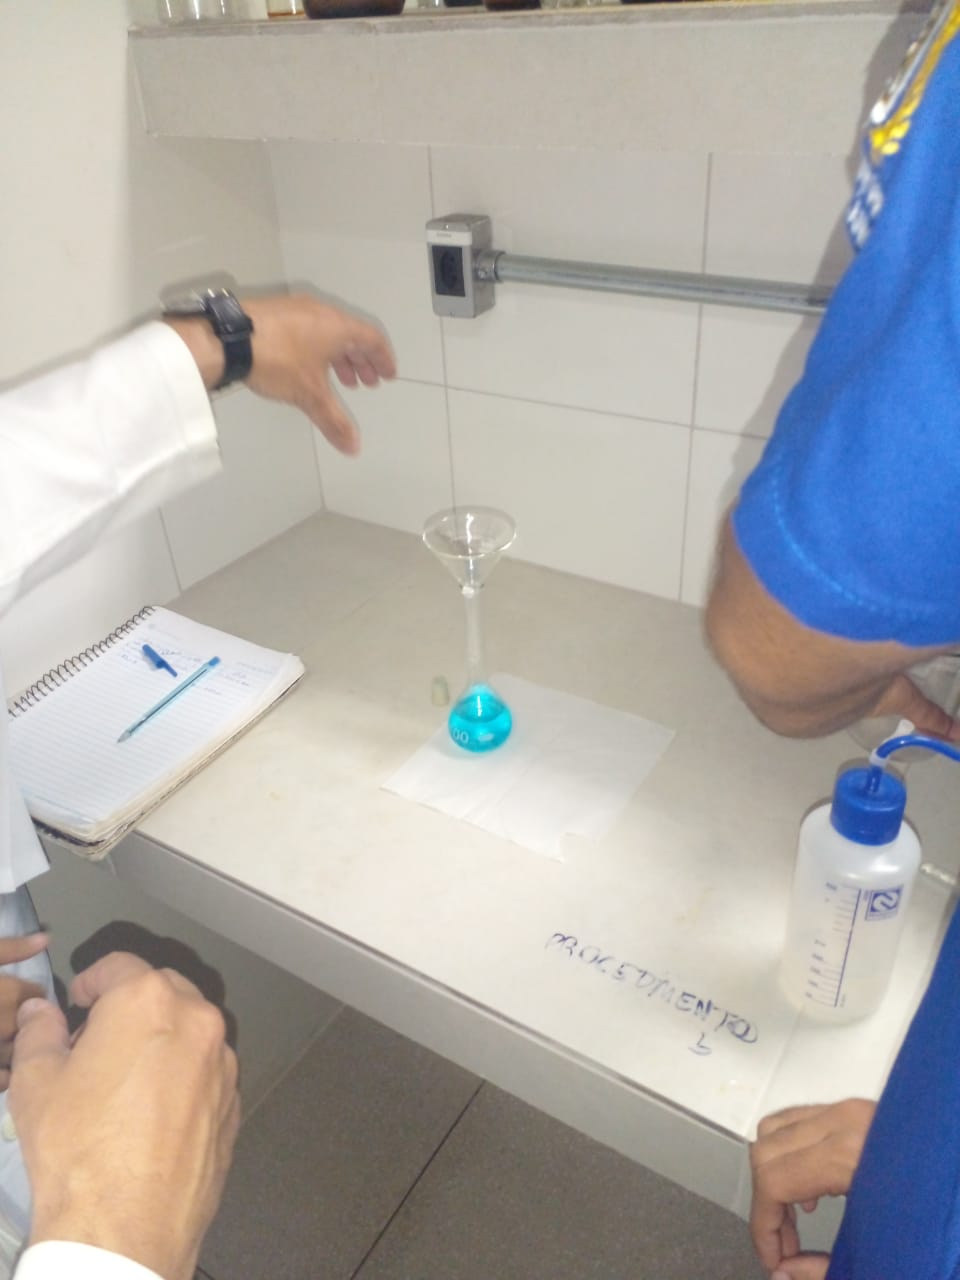
\includegraphics[scale=0.2]{04. preparo do balao.jpeg}}
            \\
            \textbf{Figura 4}: Solubilização do sulfato de cobre II\@.
            & \textbf{Figura 5}: Preparo do balão volumétrico\@.
        \end{tabular}
    \end{center}

    \doublespacing

    \indent Após a solução concentrada de sulfato de cobre II, foi realizado o processo de lavagem do becker, para
    que não houvesse resíduos do material no becker\@. O procedimento foi realizado três vezes, e a água destilada
    utilizada na lavagem, foi colocada no balão volumétrico p/ compor a solução\@.\\
    \indent Uma vez finalizado o processo de lavagem, foi adicionado mais água destilada no balão volumétrico\@.
    O procedimento foi realizado até que fosse completado os $100ml$ especificado no menisco\@.\\

    \begin{center}
        \parbox{7cm}{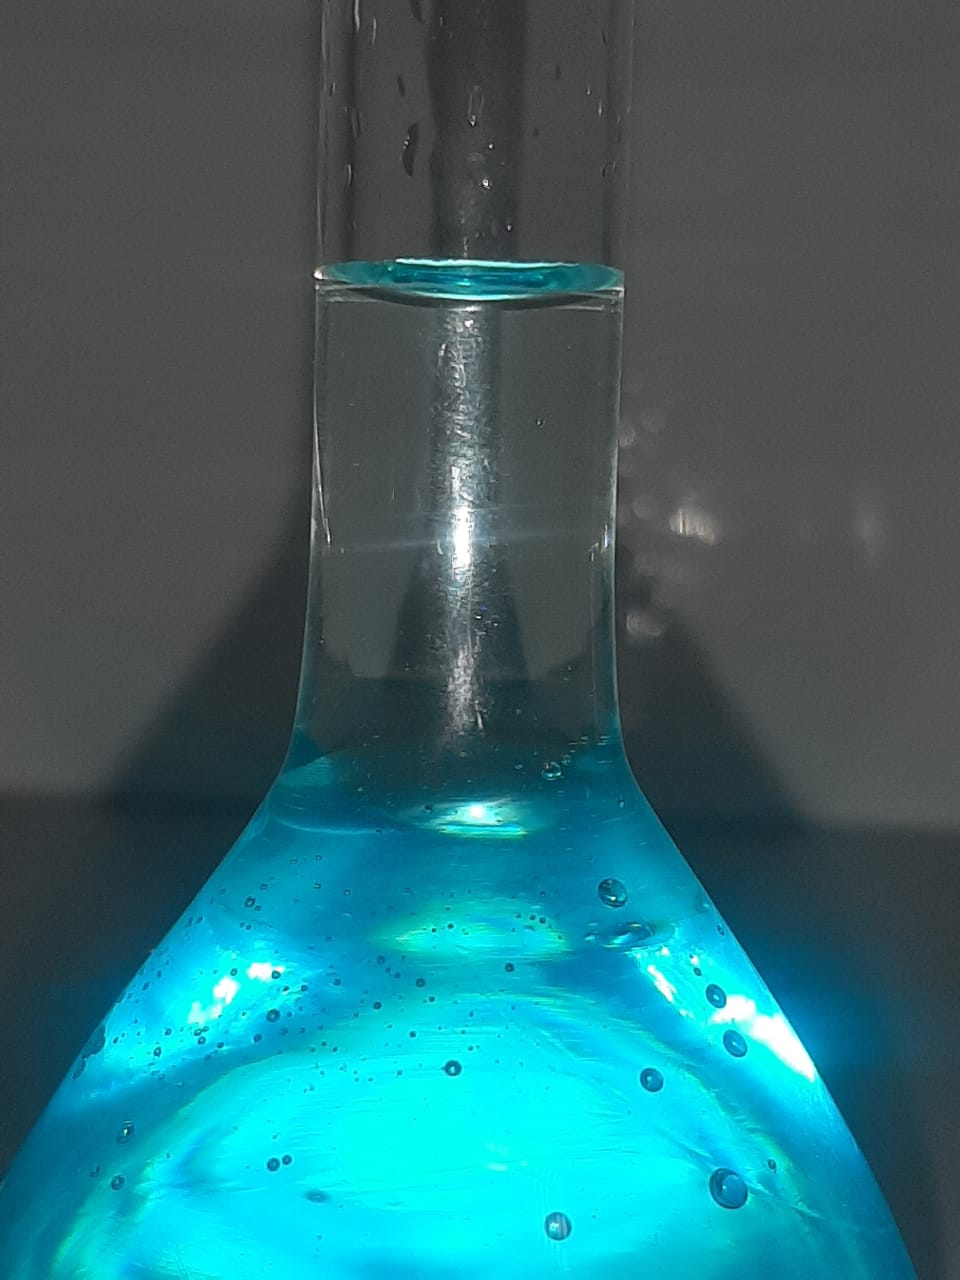
\includegraphics[scale=0.2]{06. solucao_finalizada.jpeg}}
        \singlespacing
        \textbf{Figura 6}: Solução finalizada com ajuste de nível do menisco\@.
    \end{center}
    \doublespacing

    \indent Após a finalização da solução, foi realizado o processo de homogeneização da solução\@. Tal processo foi realizado
    com a agitação da solução, até que esta se tornasse homogênea\@.\\
    \begin{center}
        \parbox{7cm}{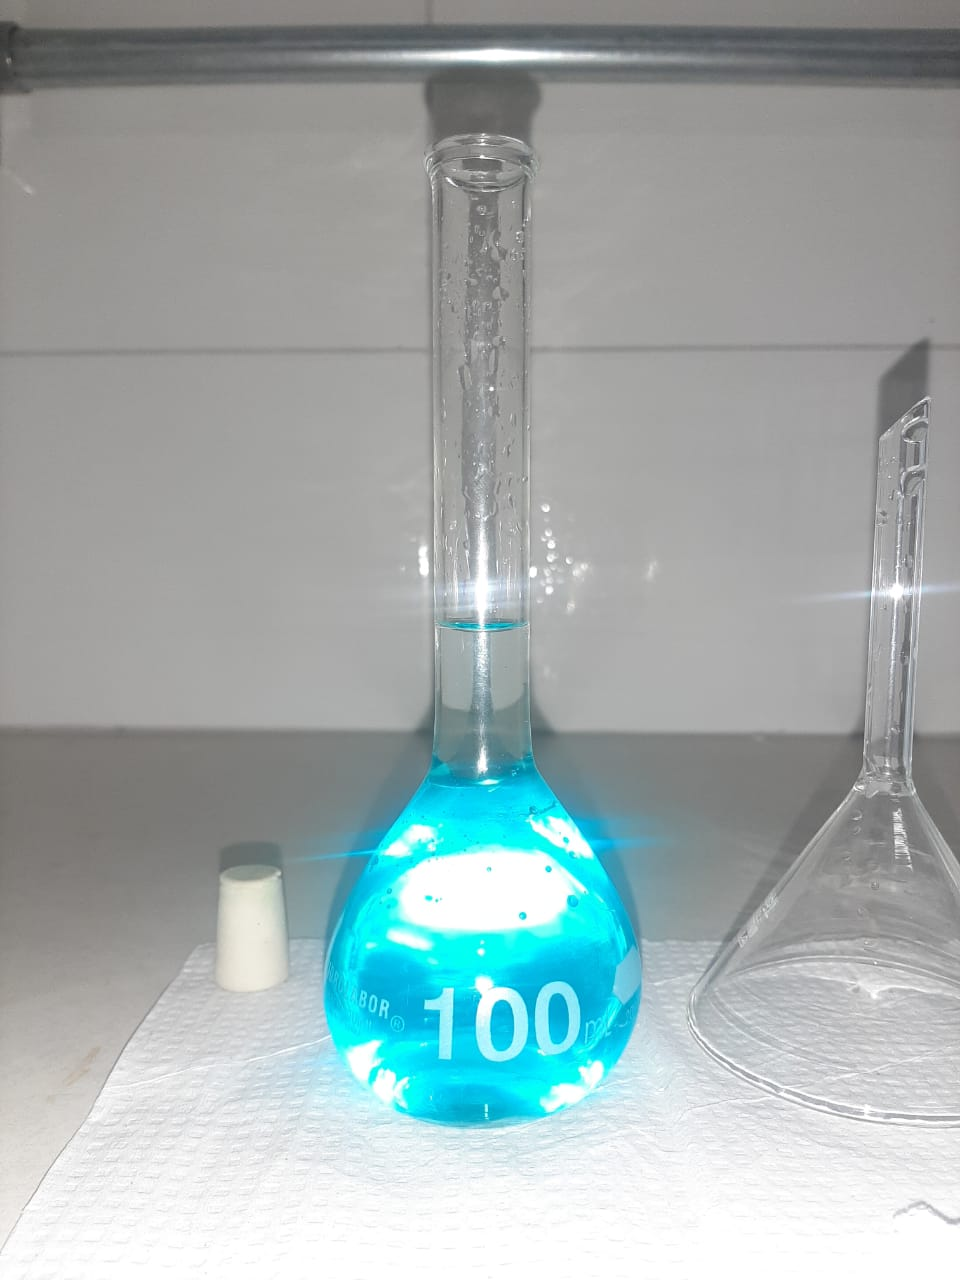
\includegraphics[scale=0.2]{10; solucao finalizada.png}}\\
        \singlespacing
        \textbf{Figura 7}: Homogeneização da solução\@.
    \end{center}
    \doublespacing

    \section{Resultados}\label{sec:resultados}
    \indent O experimento em laboratório permitiu a obtenção de uma solução de sulfato de cobre II com concentração de $0.100967\frac{g}{L}$\@.
    Tal resultado foi obtido através da equação\ref{eq:equacao_concentracao}\@.\\
    \indent O experimento careceu de detalhes sobre a precisão dos instrumentos utilizados, pois os únicos cujo o valor da incerteza associada
    conhecidos, foram os da balança e do balão volumétrico\@.\\
    \indent A incerteza associada da balança foi de $0.0001g$, e a do balão volumétrico foi de $0.01ml$\@.\\
    \indent A incerteza associada para a solução foi esperada em torno de $0.01g/L$\@. Porém, os integrantes da equipe não tomaram nota em campo,
    sendo as observações, realizadas a partir das fotos feitas do experimento e lembranças incertas do responsável por reste relatório\@.\\
    \indent A cor do sulfato de cobre II penta-hidratado é azul, tal fato é característico da presença da água na sua composição química\@.\\
    \indent A solução apresentou uma coloração azulada, devido a presença de cátions \chemfig{Cu^{2+}} na sua composição, quanto mais azul,
    mais concentrada a solução é\@.\\
    \indent O procedimento de preparo da solução pode ser descrito através da seguinte representação química\@: \\
    \begin{center}
        \schemestart $CUSO_4.5H_2O(s)+H_2O(l)$  \arrow{->}  $Cu^{2+}(aq)+S0_4^{2-}(aq)$\schemestop\par
    \end{center}
    \newpage
    \section{Conclusão}\label{sec:conclusão}
    \indent Foi possível preparar a solução de sulfato de cobre II, conforme os parâmetros e procedimentos recomendados, todos os EPI's e normas de segurança envolvidas foram preparados e aplicados durante o processo.
    \indent A equipe obteve boa experiência prática e técnica com a manipulação de instrumental e reativos químicos no processo de produção da solução, assim como dos procedimentos técnicos e práticos, registrando, anotando e realizando observações sobre cada etapa do experimento.
    \indent No mais, o Trabalho desenvolvido em grupo em reuniões e em laboratório durante o preparo das soluções trouxe resultados satisfatórios e dentro do esperado. O Relatório pôde ser elaborado sem grandes dificuldades e realizado com o devido cuidado por toda a equipe.





\end{document}\begin{figure}
    \centering
    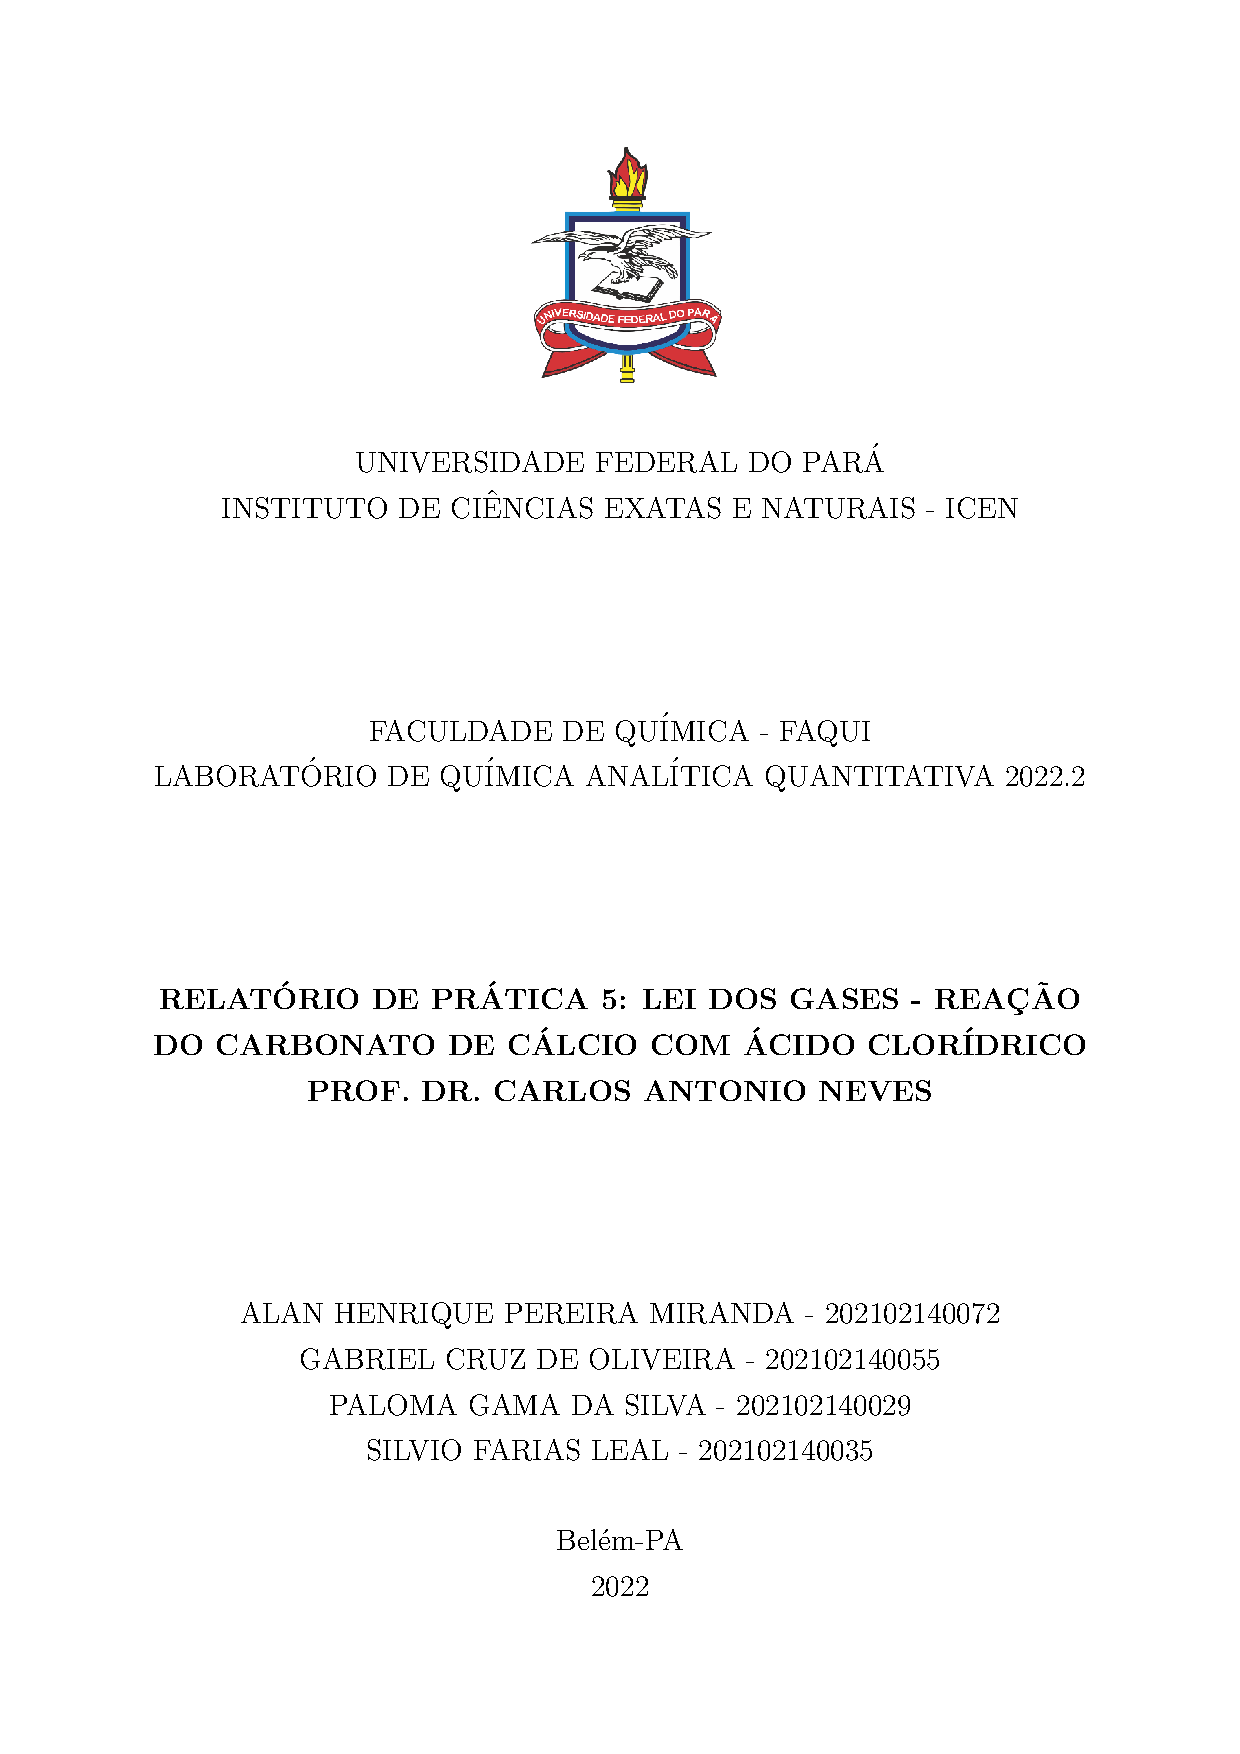
\includegraphics{/home/alan/Downloads/chemstry_article_4}
    \caption{}
    \label{fig:}
\end{figure}